% !TeX root = ../main.tex
% Add the above to each chapter to make compiling the PDF easier in some editors.

\section{Monoscopic Far-Field Rendering}
\subsection{Theory}
Monoscopic Far-Field Rendering (MFFR) is a curious approach strongly aligning with an inherent property of many optimizations in the field of rendering and real-time computing in general, which is the property of trading accuracy for speed. MFFR is a topic brought up again soon after Oculus Rift CV1's retail launch by Oculus developers Rémi Palandri and Simon Green at developer keynotes like the ARM GDC 2017 talk\cite{DiDonato.01.03.2017} and the Oculus Developer Blog as Hybrid Mono Rendering\cite{Palandri.2016}. \\
Understanding the concept requires some explanation of the technical and visual background. Proper depth perception of the human eye relies on the slight spatial distance between both eyes as each eye sees a slightly different angle of a given object. This difference in perceived angle is called stereo separation and without it, the brain has a hard to impossible time determining the depth of and at which a certain object or surface lies. Regular stereo rendering obviously recreates this separation correctly when rendering the two virtual eyes at their respective spatial offset from the HMD center - given correct projection and view matrices and accurate world scale at least. 
However, and that's one aspect MFFR exploits, as distance grows, stereo separation shrinks. In infinity, separation would be infinitely small, but even at more reasonable distances separation becomes so small that even with good vision it becomes hard to properly judge depth unless the object is large. This of course also holds true for rendered stereoscopy, but an additional limit is the pixel density of the output displays. What this means is that at a certain distance from the virtual camera, stereo separation will shrink to less than a full screen space pixel once projected. Obviously if the difference can physically not be displayed by the HMD, it seems a waste of resources to still render both eyes. \\
Mono Far-Field Rendering thus opts to skip the second view during rendering of the name-giving far field of objects. The hope here is that only rendering a single view past a certain distance reduces rendering load without the user noticing the theoretical loss in accuracy. 
This approach has caveats unfortunately. For one, the value at which a field split - the distance at which the stereo rendering is cut off and followed by only mono rendering - will depend on the individual user, their quality of vision and spatial recognition. It will also potentially depend on the resolution of the used headset given the user's vision is good enough to not deteriorate before that point. \\
Note here, this thesis will not explore these constraints of MFFR further than approximate values used for testing as time does not allow more. \\
MFFR has been implemented by Oculus LLC and Epic Games Inc in Unreal Engine 4 at some point and was recommended for example for certain types of pixel-bound mobile VR experiences with very limited GPU power, but curiously has been removed from the engine in update 4.20 without further explanation. An odd decision surely, as UE documentation posts prior to the removal indicated continued optimization efforts such as added compatibility with UE4's multiview path\cite{EpicGamesInc..2016}. 

\begin{figure}[htb]
  \centering
  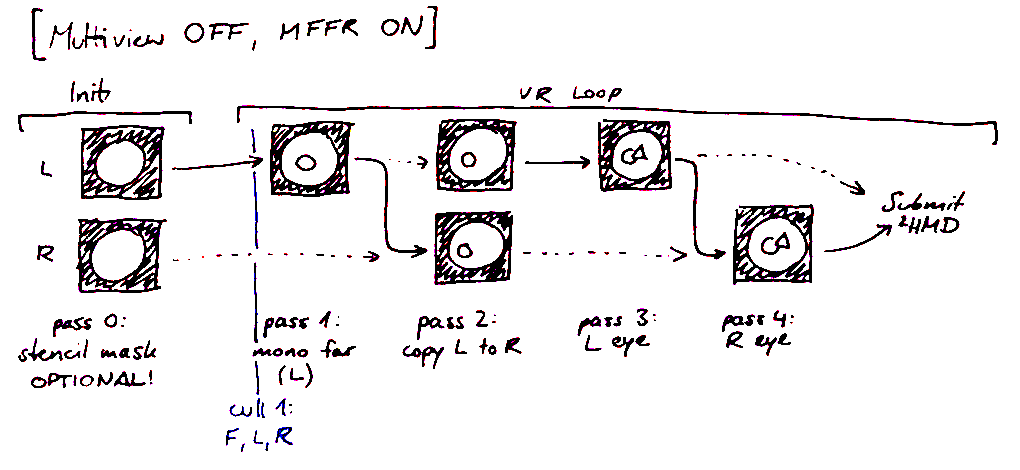
\includegraphics[width=0.9\textwidth]{pictures/flowchart_mffr}
  \caption{Far-First MFFR flowchart \textcolor{red}{[TODO: redo flowchart properly]}} \label{fig:flowchart_mffr_FarFirst}
\end{figure}

\subsection{Estimated impact}
The makeup of the scene itself will also affect effectiveness of the solution. As cautioned by Oculus LLC in their developer reference on Mono Far-Field Rendering \cite{Palandri.2016}, there is a certain baseline overhead simply for enabling the additional render pass necessary for the monoscopic image and the associated context switches. Furthermore only scenes with a significant amount of distant geometry beyond the field split distance will benefit from the optimization, as obviously the second view workload can only be saved for objects that would be contained within that second pass. \\
Going purely by Palandri and Green's blog entry, their forward-rendered UE4 implementation supposedly running on a GearVR device saw frametimes in the Epic SunTemple sample scene drop by 25\% and their best-case Unity test scene demonstrated a 49\% drop\cite{Palandri.2016}. 
This would indicate that if circumstances allow - meaning pixel-bound forward-rendered large scale scenes - impressive performance gains well upwards of 20\% can be expected, while less suitable cases in the worst case will see no change if not minor regression. 

\subsection{Implementation specifics}
Implementing Mono Far-Field Rendering into Tachyon - or any renderer for that matter - requires care and a number of changes. There are at least two possible ways of doing it, both by way of two render passes and with their own respective drawbacks and advantages. 
\subsubsection{Far-first approach}
One way of implementing MFFR is to do the far pass first in each frame, then followed by a near pass, perhaps both using the same framebuffer as illustrated in \autoref{fig:flowchart_mffr_FarFirst}. At the start of the frame, the framebuffer is cleared - only color and depth necessary - after which the far-field command buffers are submitted and executed. This pass can render directly into the buffer of one eye, then copy color and depth buffer to the other eye. Finally the near-field command buffers are submitted and render their values into the buffers already containing the far field information. \\
For this case, one extra step needs to be performed though. As the projection matrix normally projects the world as seen by the camera into a uni-cube with each axis being length 1 going from 0 to 1, and this same uni-cube is used for both depth value calculation \textit{and} projection clipping (triangle discard via clip space evaluation), the two passes can't share the same uni-cube. Ways around this would be to either use regular full-depth projection matrices and clear the depth buffer before the near pass, or to scale both passes' projection matrices by 0.5 and also translate the far projection by 0.5 so the uni-cube is split between the two fields. \\
If neither is done, the depth values of far-pass objects may appear to be closer than those of near-pass objects, effectively leading to some near-field objects being drawn \textit{behind} far ones. 
The depth buffer clear option has to benefit of utilizing full projection precision and correct triangle clipping. The matrix squashing option avoids an extra clear but will mean vertices otherwise clipped outside of the uni-cube will be pulled into the uni-cube and not skipped. \\
The overall advantage of this far-first approach then is that it yields a full precision far-field depth buffer which may be useful for stereo interpolation as briefly described in the next section \autoref{mffr_depthshift}. The disadvantage then is that early Z discard cannot be fully effective as all far geometry is rendered first, even if opaque geometry close to the camera would later obstruct it. Whether the benefits of lower split distance coupled with interpolation can outpace the additional cost of overdraw will heavily depend on the scene and how much geometry is contained within the far volume. 
The goal of this approach is to reduce memory operations and locality to a minimum and also avoid more costly compositing methods. 
\subsubsection{Near-first approach}
The obvious alternative to rendering the far pass first is of course to render the stereo near volume at the start of each frame \textcolor{red}{[TODO: mffr near first flowchart]}. A key difference to the former approach is that for near-first to work correctly, this first pass also needs to flag then stencil buffer pixel when a opaque fragment is within the uni-cube and a color value is written. Then after the stereo pass, each eye will contain a binary stencil mask of the near-field occluded screen areas. In the next step, the far pass can then execute regularly except with stencil testing enabled. This sequence has no direct need for depth buffer clearing or uni-cube sharing. The constraint, however, is that the far pass then also needs to sample from left to right eye separately as a straight buffer copy cannot work anymore. 
The obvious advantage of this approach over far-first is that early Z discard takes full effect, not to mention stencil masking may reduce the leftover areas even more. The downside is that it needs to perform additional stencil writes every frame and potentially costly sampling operations. 
\subsubsection{rtvklib MFFR}
In this case, the plan was to do far-first MFFR. It eventually became evident that for the given test scenario, this approach proved unsuccessful for various reasons. 
Before that, the theory. In the first step of each VR frame, a monoscopic render pass would render the far clip volume's color and depth values into the index 0 layer of the framebuffer. The next step would copy that layer to index 1 as well. In the final step then the regular stereoscopic render commands would be executed with reduced near field clip volume, including clearing the depth buffer at the start of the stereo pass to avoid the uni-cube issue. 
While the general approach sounds mostly straight-forward and both described ways are possible, implementing either in a Vulkan renderer is no trivial task and required the following changes to rtvklib: 
\begin{itemize}
\item for the virtual camera, a field split distance parameter is introduced and an additional frustum is added - the stereo frusta then cover the volume from near plan to split plane while the far field frustum covers split plane to far plane
\item the frustum culling procedure is altered to write the far frustum's resulting draw commands into a separate set instead of merging them into one (as would happen for regular multifrustum culling in Tachyon)
\item at initialization time of the VR render target, an additional render pass is created for monoscopy, with the main difference compared to the VR render pass being that it foregoes the multiview extension
\item add an additional set of Vulkan \codeword{VkCommandBuffer}s into which the draw commands of the far frustum cull set are to be recorded
\item add an additional set of \codeword{VkSemaphore}s to synchronize the two render passes and create them in \codeword{CreateSyncObjects()} during initialization
\item add an additional \codeword{VkCommandBuffer} for the layer copy operation
\item at initialization time of the VR render target, pre-record this copy command buffer so it can be reused every frame; this recording includes transitioning the layout of both the color and depth image from \codeword{VK_IMAGE_LAYOUT_TRANSFER_SRC_OPTIMAL} to \codeword{VK_IMAGE_LAYOUT_GENERAL}, \codeword{vkCmdCopyImage(...)} both images' layer 0 to layer 1 and then transition the layouts in reverse again
\item in the per-frame recording procedure of the VR render target, \codeword{RecordCommandBuffers(...)}, the entire structure of begin and end of command buffers and render pass and per-pipeline \codeword{RecordDrawCommand(...)} calls is duplicated with the monoscopy render pass and far field command buffers set; after that block the prior regular stereo recording still takes place
\item in the render target's \codeword{RenderFrame(...)} function the far field command buffer and layer copy command buffer submission is inserted before the regular stereo submits; the mono submit is set to wait on \codeword{mRenderCompleteSemaphores} and signal \codeword{mFarfieldCompleteSemaphores}, the latter of which the stereo submit is set to wait on
\item in VR render target's camera setup, construct the far field frustum projection matrix as outlined in \cite{Lapinski.2017} pp. 515-519 - transposed as Tachyon still retains OpenGL matrix format for a few matrix types
\item add an additional set of camera data struct and camera index
\item in the render target's \codeword{UpdateCameras()} call, update the far field volume's view projection matrix by transforming aforementioned projection matrix by the current HMD pose and write that updated matrix to the camera data buffer on the GPU
\end{itemize}
\textcolor{red}{[TODO: sort this list a bit better? normal text some of it?] \\}

Some issues with this implementation do prevail and make it unfit for productive deployment in Tachyon yet, unfortunately. 
For one, the projection and view matrices used for the far field remain incorrect and sufficiently accurate projection math could not be determined in time, so head rotation leads to incorrect separation effects on the horizontal axis. And while the lack of pure separation at little to no sideways tilt may be acceptable and not easily noticed, tilting the head means more severe separation mismatch as the spatial disconnect is expanded from being mostly horizontal to being horizontal and vertical. \\
Another issue is that Vulkan render passes by default discard fragments at the their end if depth testing is enabled and the depth value of said fragment equals 1.0 and is thus on the far plane. This meant any color values written by the far pass and not overwritten by the near pass would be discarded right at the end of the stereo pass and before presentation. A workaround for this was to clear the depth buffer at the start of the stereo pass not to 1.0 but to 0.999999 (22 of 23 mantissa bits set to 1), the closest value a IEEE-754 float can reach below 1.0. With this tweak, color values were correctly composited together without any visible loss at the near field's split plane. \\
Lastly, and most importantly, performance simply was not up to par. On the i7 and RTX2080 test system, \textit{enabling} MFFR with a sufficiently far split distance yielded a 34\% performance \textit{loss}. The culprit for this most likely two-fold. One factor is the detrimental Z ordering of the submitted draw commands, as much of the far field color buffer is overwritten by the near pass and thus counts as wasted effort. The other factor is the lack of parallelism due to the use of a shared framebuffer. The two render passes need to be synchronized to run in order and cannot be scheduled on parallel warps to increase GPU utilization and thus performance. \\
As such, the rtvklib MFFR implementation as presented here remains beneficial only in theory and will require further work - if not a complete overhaul to near-first approach - to result in real performance gain. \\

\textcolor{red}{[TODO: example picture comparison]}



\subsection{MFFR Variant: Depth Shift}  \label{mffr_depthshift}
MFFR in its basic version as described above obviously completely foregoes separation beyond the split distance and as such that split distance has to be set relatively far back to minimize the visual inaccuracy. So naturally it seems profitable to attempt to try and reduce that split distance closer to the camera by artificially increasing that accuracy again. One such way is to use the data already contained in the framebuffer's depth layer during rendering. 
As stereo separation is mostly dependent on depth given the object itself and its properties are known, it is logical to approximate small amounts of separation based on that depth buffer. 
Instead of simply copying layer 0 to layer 1 after the far field pass, one can do a sampling pass over layer 1 from layer 0 or a post-processing pass after the copy operation and slightly shift pixels according to the depth value of the respective given fragment. \\
This interpolation should allow pulling the field split distance closer to the camera and save some stereo render time, however it is unclear whether the savings outweigh the additional processing cost and this thesis did not explore MFFR beyond the base variant. \\

\textcolor{red}{[TODO: shift math or geometric illustration]}

\subsection{MFFR Variant: Alternate eye}
Another possible way of pulling in the split distance value while retaining approximated separation comes back to the VR property of high framerate as underlying for earlier chapters like the Round Robin Culling. 
Assuming high framerate and refresh rate, the mono render pass could be called with the camera parameters not custom calculated as a middle point between the two eyes but alternating between left and right eye parameters each frame. This way each alternating eye would be correctly projected every other frame and incorrect data would likewise also only persist for one frame at a time in each eye. \\
If this eye-alternating MFFR were to be combined with interpolation of the respective incorrect eye, the perceived inaccuracy (seen as flickering as the visual information is only incorrect every other frame) may be further reduced. Candidates for this are a single frame temporal reconstruction, although a single previous frame may not be enough for good results, or a simple frame interpolation. \\
Once again this thesis does not encompass this additional option and thus it is unknown how far the split distance could be pulled in and whether related savings would outweigh interpolation cost. And just as with Round Robin Culling, the same potential artifacts and issues are present here. 
